
\section{Experiments}

% \subsection{Datasets}
% \subsection{Metrics}
\subsection{Experimental Setup}
\noindent \textbf{Implementation Details.} Tora is initialized with OpenSora v1.2 weights, and training videos have resolutions from 144p to 720p and frame counts ranging from 51 to 204. To balance training FLOP and memory usage, we adjust the batch size from 1 to 50. We use Adam Optimizer~\cite{DBLP:journals/corr/KingmaB14} with a learning rate of $2\times10^{-5}$ on 8 NVIDIA A100. The 3D VAE is initially trained on datasets ~\cite{DBLP:conf/cvpr/MehlSJNB23,DBLP:conf/cvpr/MayerIHFCDB16,DBLP:journals/ijcv/RanjanHTTRB20,DBLP:journals/corr/abs-2001-10773} for optical flow estimation and then frozen during Tora training. We train Tora for 2 epochs with dense optical flow and fine-tune for 1 epoch with sparse trajectories. The maximum number of sampling trajectories $N$ is set to 16. The inference step and the guidance scale are set to 30 and 7.0, respectively.

\noindent \textbf{Dataset.} Our training videos are sourced from four datasets: 1) Panda-70M~\cite{DBLP:journals/corr/abs-2402-19479}, from which we use the training-10M subset containing high-quality videos; 2) Mixkit~\cite{mixkit}; 3) Pexels~\cite{pexel}; and 4) Internal videos. The internal videos are manually annotated, with each clip labeled to include object masks and camera movement. Following our data processing pipeline, we select about 630k eligible videos for the training dataset. For inference, we curate 185 clips with diverse motion trajectories and scenes, to serve as a new benchmark for evaluating the motion controllability. 
%Additional dataset details for training Tora and the 3D VAE can be found in our supplementary materials.

\noindent \textbf{Metrics.} We leverage standard metrics including Fréchet Video Distance (FVD)~\cite{Thomas2018fvd}, and CLIP Similarity (CLIPSIM)~\cite{wu2021godiva} to quantitatively evaluate video quality. 
%For assessing motion controllability, we leverage Trajectory Error~(TrajError), which computes the average L1 distance between the generated and pre-defined trajectories.  A human evaluation of DiT-based methods is also provided in the supplementary materials because of space limitations.
For assessing motion controllability, we utilize the Trajectory Error (TrajError) metric, which calculates the average L1 distance between the generated and predefined trajectories. 
%Additionally, the mean Intersection over Union (mIoU) is employed to compare the generated objects with the ground truth, as determined by SAM2~\cite{ravi2024sam2segmentimages}, to comprehensively assess the overall movement of the subjects.





\subsection{Results}

\begin{table*}[!t]\small
\setlength{\tabcolsep}{3pt}
% \renewcommand{\arraystretch}{1.1}
\centering
\begin{tabular}{ccccccccccccc}
\toprule
\multirow{2}{*}{Method} & \multicolumn{3}{c}{FVD~($\downarrow$)} & \multicolumn{3}{c}{CLIPSIM~($\uparrow$)} & \multicolumn{3}{c}{TrajError~($\downarrow$)} \\ \cmidrule(lr){2-4} \cmidrule(lr){5-7} \cmidrule(lr){8-10}
 & 16-frame & 64-frame & 128-frame & 16-frame & 64-frame & 128-frame & 16-frame & 64-frame & 128-frame \\ 
\midrule
\rowcolor{black!10} \multicolumn{1}{l}{\textbf{\textit{UNet-based method}}} &&&&&&&&& \\
VideoComposer~\cite{wang2023videocomposer} & 529 & 668 & 856 & 0.2335 & 0.2284 & 0.2236 & 15.11 & 29.14 & 58.76    \\
DragNUWA~\cite{yin2023dragnuwa} & 475 & 593 & 784 & 0.2385 & 0.2341 & 0.2305 & 10.04 & 17.33 & 41.25    \\
AnimateAnything~\cite{DBLP:journals/corr/abs-2311-12886} & 487 & 602 & 775 & 0.2399 & 0.2342 & 0.2313 & 13.39 & 27.28 & 51.33     \\
TrailBlazer~\cite{DBLP:journals/corr/abs-2401-00896} & 459 & 581 & 756 & 0.2403 & 0.2351 & 0.2322 & 11.68 & 19.47 & 44.10    \\
MotionCtrl~\cite{wang2024motionctrl} & 463 & 572 & 731 & 0.2412 & 0.2376 & 0.2331 & 9.42 & 16.46 & 38.39  \\
\midrule
\rowcolor{black!10} \multicolumn{1}{l}{\textbf{\textit{DiT-based method}}} &&&&&&&&&\\
OpenSora~\cite{OpenSora} & \textbf{430} & 476 & 533  & \textbf{0.2452} & 0.2433 & 0.2411 & 286.43 & 321.52 & 373.17         \\
OpenSora-based DragNUWA*  & 451 & 504 & 565  & 0.2430 & 0.2419 & 0.2393 & 10.11 & 13.88 & 21.75     \\
\textbf{Tora(Ours)} & 438 & \textbf{460} & \textbf{494} & 0.2447 & \textbf{0.2435} & \textbf{0.2418} & \textbf{7.23} & \textbf{8.45} & \textbf{11.72}     \\ 
\bottomrule
\end{tabular}
\caption{
%Quantitative comparisons with state-of-the-art motion-controllable video generation models. As the number of generated frames increases, Tora demonstrates a growing performance advantage over the UNet-based methods, maintaining a high degree of stability in trajectory control.
Quantitative comparisons with motion-controllable video generation models. As the number of generated frames
increases, Tora's performance advantage over UNet-based methods becomes more pronounced. Specifically, Tora not only enhances motion fidelity but also improves the visual quality of the foundational model. Comparisons with OpenSora-based DragNUWA highlight the strengths of our proposed motion modules, which integrate seamlessly with DiT’s architecture.}
\label{tab1}
\vspace{-1mm}
\end{table*}

% We compare our method with popular motion-guided video generation approaches in three settings: 16, 64, and 128 frames, all at a resolution of 512 × 512 for a fair evaluation. The provided trajectories are adjusted to fit the different video lengths. For most U-Net-based methods, we use sequenced inference, where the last frame generated from one batch serves as the visual condition for the next, aligning with their inference strategies. As shown in Table~\ref{tab1}, in the 16-frame setting typical for U-Net methods, MotionCtrl and DragNUWA align better with the provided trajectories but still fall short compared to our proposed Tora. With an increasing number of frames, U-Net methods exhibit significant deviations, leading to misalignment errors that result in deformations, motion blur, or object disappearance in later sequences. In contrast, Tora remains highly robust across varying frame counts due to the transformer's scaling abilities. In the 128-frame test setting, Tora's trajectory accuracy surpasses other methods by 3 to 5 times, showcasing its outstanding motion control capabilities. Figure~\ref{fig:5} presents an analysis of Trajectory Error across different resolutions and durations. Unlike U-Net models, which exhibit substantial trajectory errors over time, Tora shows only a gradual increase in error as duration extends. This aligns with the decrease in video quality observed in the DiT model. The results demonstrate that our method effectively maintains trajectory control over longer durations.

We evaluate against motion-guided video generation methods using 16-frame, 64-frame, and 128-frame configurations. Trajectories are scaled proportionally for different durations. UNet-based approaches utilize sequential inference for extended generation. Since there are no DiT-based methods, we adapt DragNUWA's motion trajectory design to our foundation model as an additional baseline. Specifically, we implement its official convolutional motion feature extraction and linear projection-based injection. To ensure compatibility with base DiT model, we perform downsampling across both spatial and temporal dimensions.

As shown in Table~\ref{tab1}, UNet-based methods all exhibit increasing deviations with longer sequences, causing motion blur and object deformation. In contrast, Tora leverages the transformer's scaling capabilities to maintain robustness, achieving 3-5 times higher trajectory accuracy and approximately 30-40$\%$ better FVD in 128-frame tests. Figure~\ref{fig:6} shows a comparative qualitative analysis of Tora against these mainstream motion control techniques.

While the OpenSora achieves high visual quality, its inability to incorporate motion control leads to random object trajectories, resulting in significantly elevated TrajError. Notably, Tora demonstrates dual superiority over OpenSora in both motion control efficacy and visual performance at most settings. We find Tora's exceptional capacity in suppressing temporal artifacts and motion blurring compared with OpenSora (see Appendix for visual comparisons), yielding enhanced temporal coherence and video stability. While OpenSora-based DragNUWA improves motion controllability over UNet-based methods, its motion representations exhibit intrinsic incompatibility with DiT's latent space. This architectural incompatibility induces suboptimal feature integration during training, consequently degrading visual quality by about 5$\%$ below baseline. 
%Through systematic alignment with DiT, our motion modules enable seamless motion control integration that simultaneously preserves visual fidelity and enhances spatiotemporal stability.

\begin{figure}[!t]
    \centering
    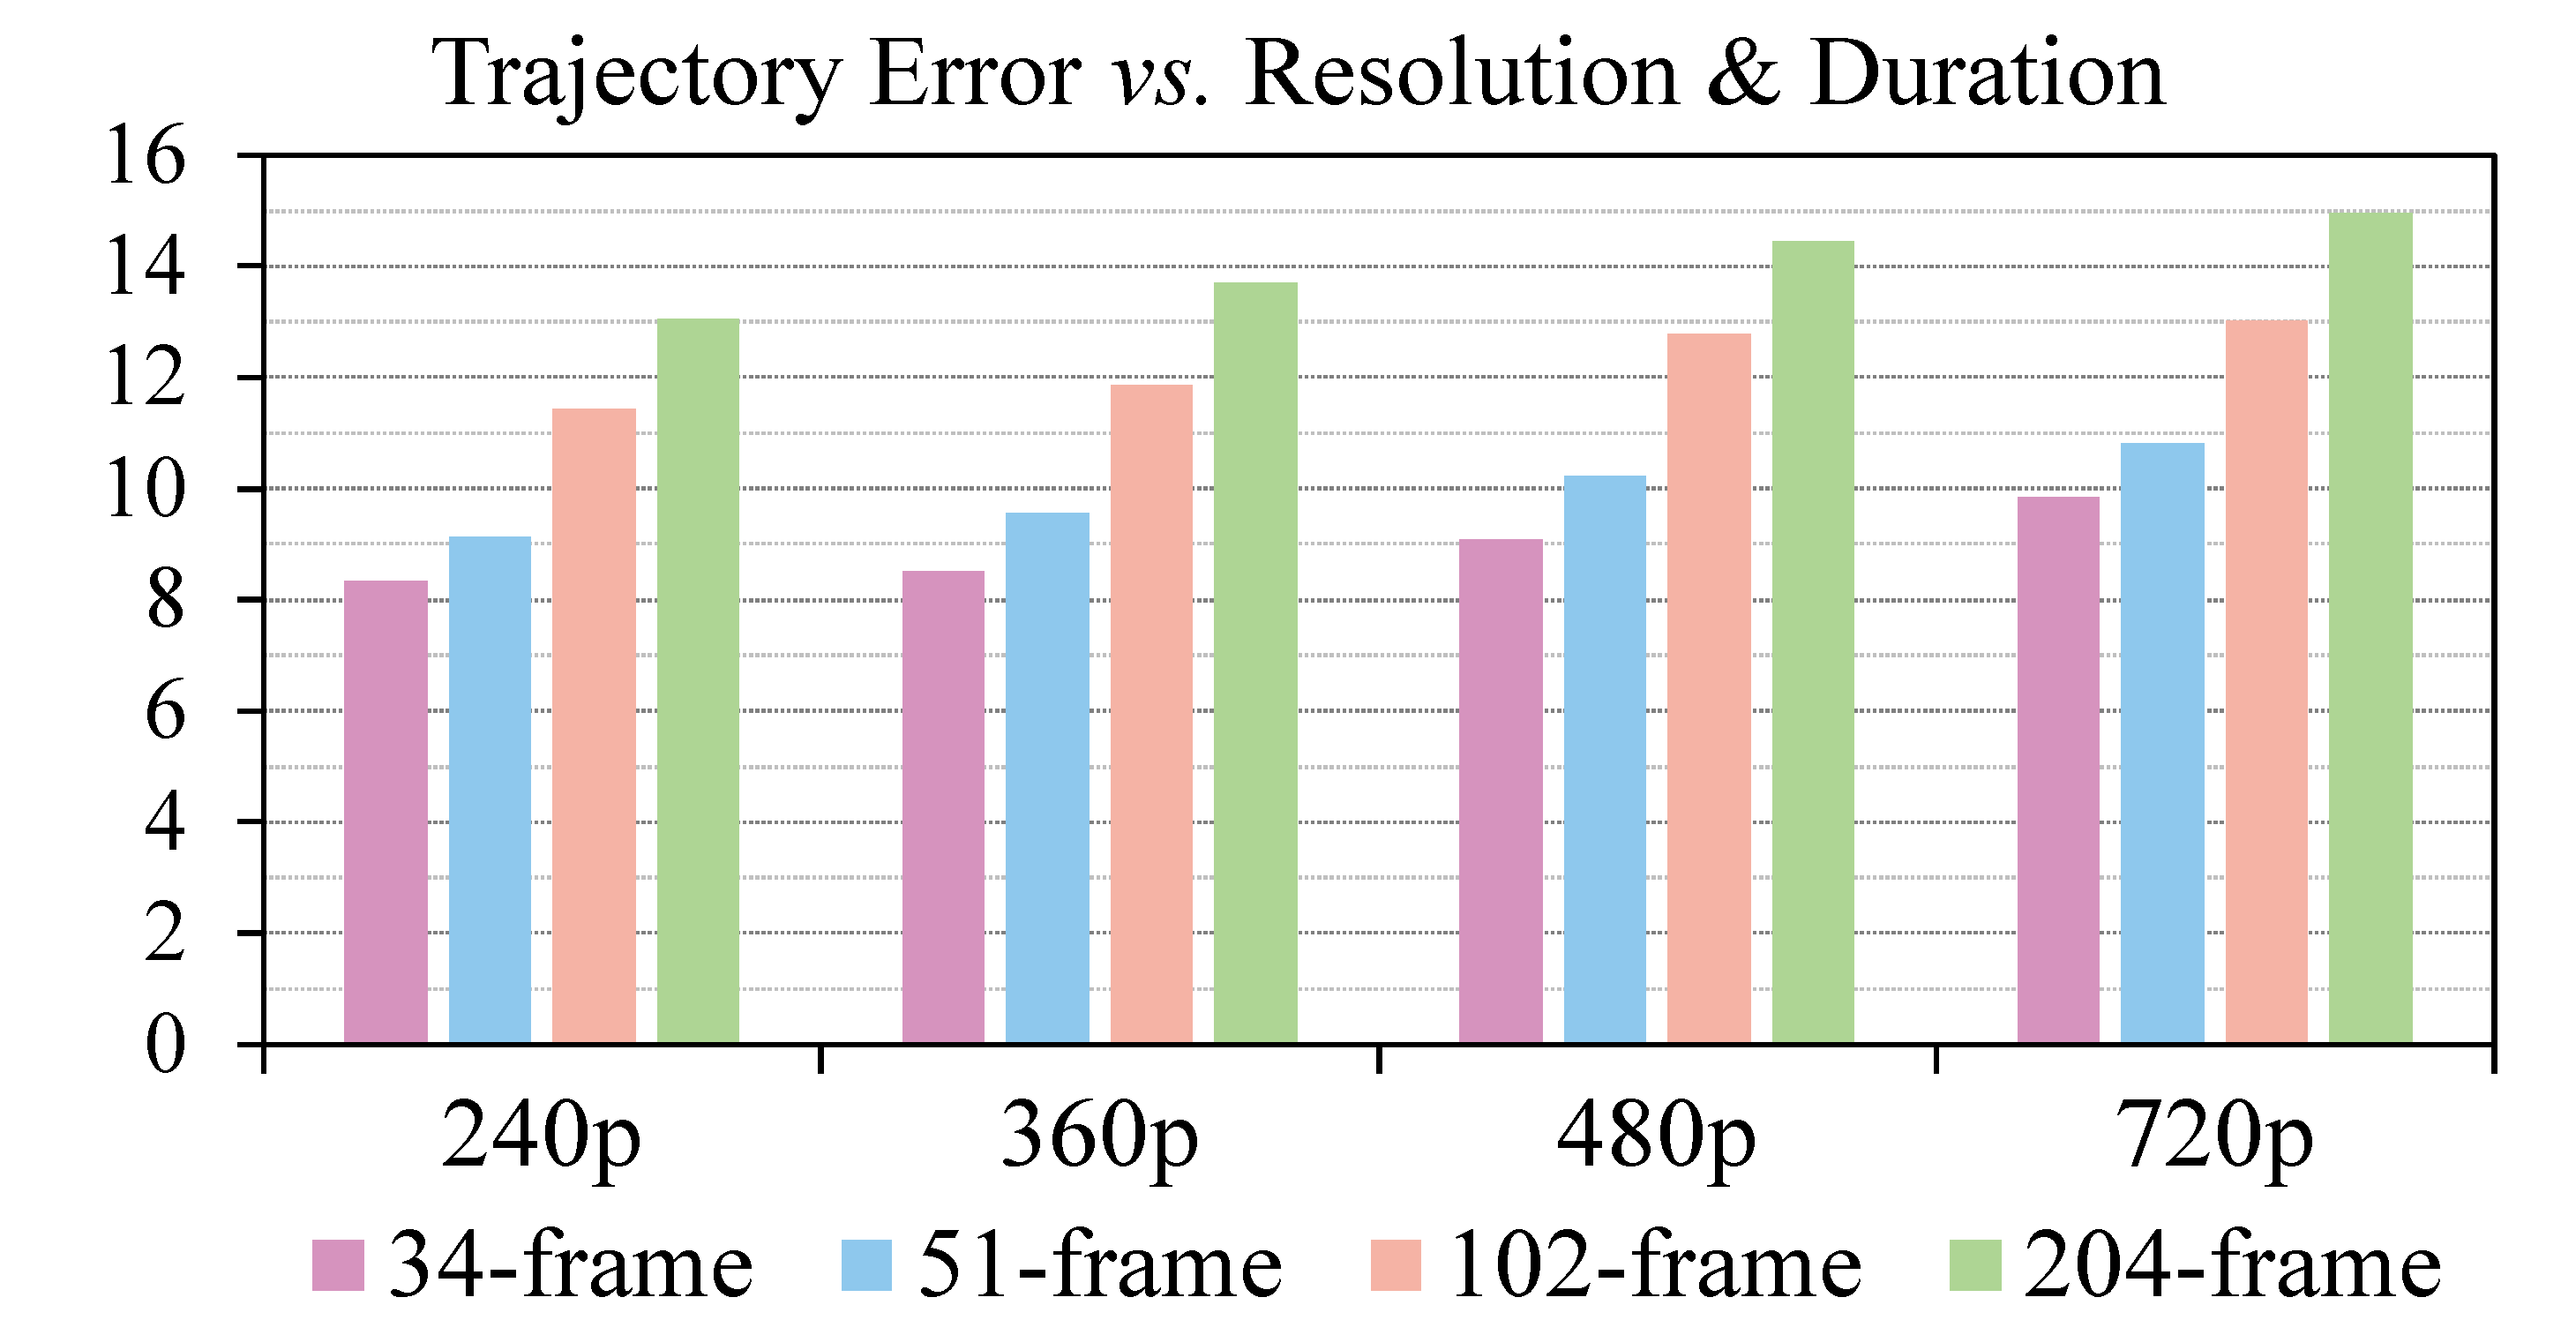
\includegraphics[width=0.45\textwidth]{images/dz.pdf}
    \caption{
        Comparison of Trajectory Error across various resolutions and durations. %Unlike UNet-based models, our method maintains motion control with a gradual increase in error.
    }
    \label{fig:5}   
\end{figure}

Figure~\ref{fig:5} presents an analysis of Trajectory Error across different resolutions and durations. Unlike UNet models, Tora shows a gradual increase in error as duration extends. This aligns with the decrease in video quality observed in the DiT model. The results demonstrate that our method effectively maintains trajectory control over longer durations.



\begin{table}[!t]\footnotesize
\centering
% \setlength{\tabcolsep}{2.5pt}
\renewcommand{\arraystretch}{1.1}
\begin{tabular}{cccc}
    \toprule
    Method             & FVD~($\downarrow$) & CLIPSIM~($\uparrow$) & TrajError~($\downarrow$) \\ \midrule
    Sampling Frame &  581   &  0.2304       &    27.61              \\
    Average Pooling    &  558   &  0.2325    &          20.97       \\
    3D VAE             &  \textbf{513}   &  \textbf{0.2358}       &   \textbf{14.25}               \\ 
    \bottomrule
\end{tabular}
\caption{Evaluation of the impact of different trajectory compression methods.} 
\vspace{-3mm}
%The 3D VAE yields superior results in motion-conditioned encoding.}
\label{tab2}
\end{table}

%We compare our method against prevalent motion-guided video generation approaches. The evaluation is conducted under three settings: 16, 64, and 128 frames, all with a resolution of 512 $\times$ 512 for fair comparison. The provided trajectories are clipped to accommodate different evaluated video lengths. For most U-Net based methods, we employ sequenced inference, wherein the last frame generated by the previous batch serves as the visual condition for the current batch, aligning with their inference settings. As illustrated in Table~\ref{tab1}, under the 16-frame setting commonly employed by U-Net based methods, MotionCtrl and DragNUWA exhibit better alignment with the provided trajectories but are still weaker compared to our proposed Tora. As the frame count increases, the U-Net based methods show significant deviations in certain frames, with misalignment errors propagating and leading to deformation, motion blur, or object disappearance in subsequent sequences. In contrast, Tora demonstrates high robustness to varying frame numbers due to the integration of the transformer's scaling ability. When evaluated under the 128-frame test setting, Tora's trajectory accuracy surpasses other methods by a factor of 3 to 5, demonstrating its exceptional motion control capabilities. In Figure~\ref{fig:5}, we provide an analysis of the Trajectory Error across varying resolutions and durations. Unlike U-Net based models, which exhibit significant trajectory errors over time, Tora shows only a gradual increase in Trajectory Error as duration increases. This gradual increase in error aligns with the decrease in video quality observed in the DiT model as the duration extends. The results clearly indicate that our method maintains effective trajectory control over longer durations.

% Please add the following required packages to your document preamble:

\begin{figure*}[!t]
    \centering
    \includegraphics[width=0.95\textwidth]{images/compare_vis.pdf}
    \caption{
        Qualitative Comparisons on Trajectory Control. 
        %Tora not only adheres precisely to the specified trajectory but also produces smoother movement that conforms to the physics world. Please visit our supplementary materials for detailed video results.
        In the bicycle scenario, Tora realistically captures pedaling motions, while other methods show legs in an unnatural, nearly horizontal position. In another case, DragNUWA causes significant deformation of the lanterns, and MotionCtrl fails to accurately depict two lanterns. Overall, Tora not only adheres precisely to the specified trajectory but also produces smoother movement that conforms to the physical world. 
    }
    \label{fig:6}   
    \vspace{-2mm}
\end{figure*}

% Figure~\ref{fig:6} shows a comparative analysis of our proposed method against mainstream motion control techniques. In the bicycle scenario, the human legs produced by our method demonstrate realistic pedaling motions, while DragNUWA's output unrealistically depicts legs in a nearly horizontal position. Additionally, both DragNUWA and MotionCtrl exhibit pronounced motion blur towards the end of their videos.  In another scenario, DragNUWA causes significant deformation of the lantern due to continuous trajectory changes, whereas MotionCtrl, despite producing a relatively accurate trajectory, does not achieve the expected depiction of two lanterns. Overall, our approach closely follows the given trajectories and minimizes object deformation, ensuring higher fidelity in motion representation.




\subsection{Ablation study}
%We conduct several ablation studies to analyze the effects of our design choices. All models are evaluated using 480p resolution, a 16:9 aspect ratio, and 204 frames.




\noindent \textbf{Trajectory Compression.} To validate the alignment of motion patches with the DiT inputs, we explore three different methods for trajectory compression, as summarized in Table~\ref{tab2}. The first method samples the mid-frame as a keyframe for successive 4-frame intervals and uses Patch-Unshuffle~\cite{jang2023pucapatchunshufflechannelattention} for spatial compression. While simple, this approach is sub-optimal for motion control due to potential flow estimation errors during rapid movements or occlusions, and the increased dissimilarity between patches complicates learning. The second method employs average pooling to gather information from successive frames. Although this captures a general sense of movement, it sacrifices precision by averaging the trajectory's direction and magnitude, diluting important motion details. Our method utilizes a 3D motion VAE to extract the global context of successive trajectory intervals. 
%The trajectory data is converted into RGB images to leverage existing 3D VAE weights.
Extensive training on a large dataset of trajectory videos with this method yields the best results, highlighting the effectiveness of our customized VAE approach for compression.




% To incorporate the trajectory vector within the same latent space as video patches, we investigate three distinct methods for trajectory compression, as summarized in Table~\ref{tab2}. The first method samples the mid-frame as the keyframe for successive 4-frame intervals and employs patch-unshuffle for spatial compression. Despite its simplicity, this method proves sub-optimal for motion control, primarily due to the potential flow estimation errors when encountering rapid motions or occlusions. Additionally, the magnified dissimilarity between patches induced by the chosen frame interval exacerbates learning challenges. The second method utilizes average pooling to gather successive frames. While this captures a general sense of movement, it inadvertently sacrifices precision by homogenizing the trajectory's direction and magnitude, thereby diluting critical motion details. To preserve the trajectory information between consecutive frames as much as possible, we further employ a 3D VAE to extract the global context of successive trajectory intervals. The trajectory data is visually translated into an RGB image format to leverage existing 3D VAE weights.  Extensive training on a large scale of trajectory videos with this setup yields the most favorable outcomes, underscoring the efficacy of our tailored 3D VAE approach in trajectory compression.

\begin{table}[!t]\footnotesize
\centering
% \setlength{\tabcolsep}{2.5pt}
\renewcommand{\arraystretch}{1.1}
\begin{tabular}{cccc}
\toprule
Method             & FVD~($\downarrow$) & CLIPSIM~($\uparrow$) & TrajError~($\downarrow$) \\ \midrule
Extra Channel &   542  &    0.2329     &   21.07               \\
Cross Attention    &   526  &    0.2354     &   18.36               \\
Adaptive Norm        & \textbf{513}    &   \textbf{0.2358}     & \textbf{14.25}                 \\ 
\bottomrule
\end{tabular}
\caption{Different variants of motion fusion blocks employed in MGF. Adaptive Norm works best.}
\label{tab3}
\vspace{-3mm}
\end{table}

\noindent \textbf{Block design and integrated position of MGF.} We train the three variant MGF blocks as previously described, with the results presented in Table~\ref{tab3}. Notably, the adaptive norm block achieves lowest FVD and Trajectory Error, while also exhibiting the highest computational efficiency. This advantage arises from its ability to dynamically adapt features based on varying conditions without strict alignment, a common cross-attention challenge. It also maintains temporal consistency by modulating conditional information over time, essential for incorporating motion cues. In contrast, channel concatenation can lead to information congestion, making motion signals less effective. We find that initializing the normalization layer as the identity function is vital for optimal performance. Additionally, placing the MGF module within the Temporal DiT block significantly enhances trajectory motion control, evidenced by a drop in Trajectory Error from 23.39 to 14.25. %This setup improves the MGF's interaction with temporal dynamics, enhancing motion synthesis fidelity.

\begin{table}[!t]\footnotesize
\centering
% \setlength{\tabcolsep}{2.5pt}
%\renewcommand{\arraystretch}{1.1}
\begin{tabular}{ccccc}
\toprule
Motion-guidance            & FVD~($\downarrow$) & CLIPSIM~($\uparrow$) & TrajError~($\downarrow$) \\ 
\midrule
Dense Flow &   601  &      0.2307   &               39.34   \\
Sparse Flow  &  556   &    0.2334    &        24.73          \\
Hybrid             &  \textbf{513}   &  \textbf{0.2358}       &   \textbf{14.25}               \\ 
\bottomrule
\end{tabular}
\caption{Ablation of the type of training trajectories. ``Hybrid" denotes the two-stage training strategy.}
\label{tab4}
\vspace{-3mm}
\end{table}


\noindent \textbf{Training Strategies.} We evaluate the two-stage training approach, with results in Table~\ref{tab4}. Training only with dense optical flow is ineffective, as it fails to capture the details of sparse trajectories. Conversely, using only sparse trajectories provides limited information, complicating the learning process. In contrast, our two-stage strategy demonstrates better adaptability and versatility in managing various motion patterns, leading to improved overall performance.




% \begin{table}[]\footnotesize
% \centering
% \setlength{\tabcolsep}{2.5pt}
% \renewcommand{\arraystretch}{1.1}
% \begin{tabular}{cccc|cc}
% \hline
% TE                           & MGF                  & TSA                  & SSA                   & FVD                  & Trajecoty Error      \\ \hline
%  \checkmark  &                  \checkmark     &                      &                       &         556             &          23.44            \\
%     \checkmark                          &   \checkmark                    &    \checkmark                   &                       &      513                &   14.25                   \\
% \checkmark          & \checkmark  & \checkmark  & \checkmark  & 521 & 16.14 \\ \hline
% \end{tabular}
% \caption{Ablation of different compression methods.}
% \end{table}



\noindent \textbf{Scaling motion-control ability.} We investigate scaling laws in motion-controllable video generation by examining model parameter size and training volume. To leverage existing multi-size foundational models, we transfer our motion modules to CogVideoX architectures (2B/5B parameters), resulting in Tora-CogVideoX2B (2.5B) and Tora-CogVideoX5B (6.3B). Our implementation retains base VAE for motion compression while inserting MGF prior to Expert Transformer's full attention module. Figure~\ref{f1} demonstrates that increasing model scale and training data improves motion control well, confirming our modules' seamless compatibility with DiT's scalability framework.

\begin{figure}[!t]
    \centering
    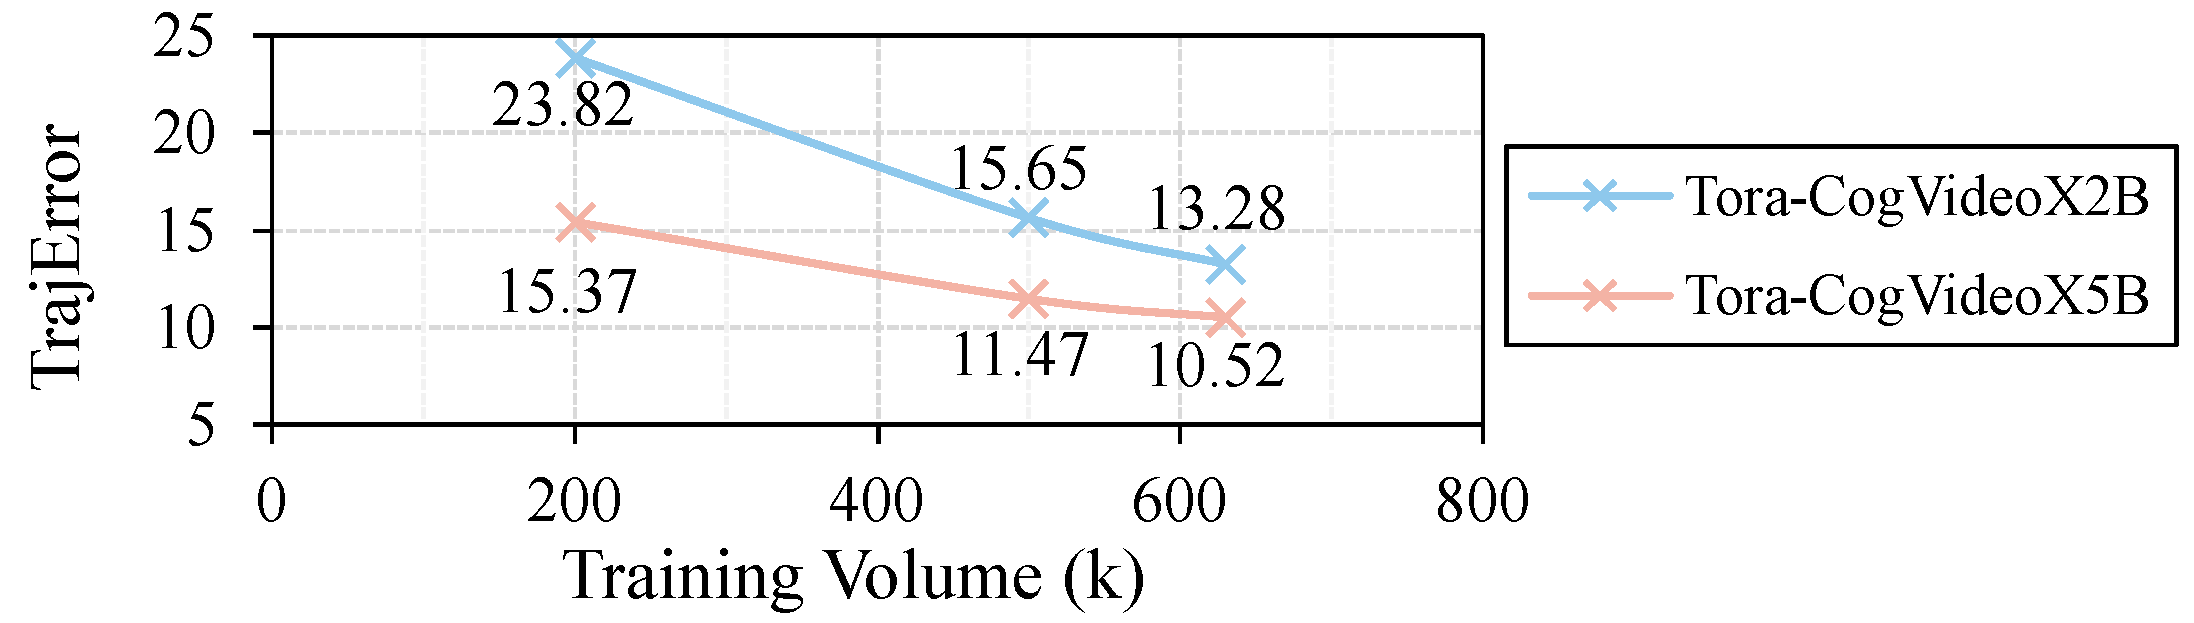
\includegraphics[width=1\linewidth]{images/reb-f1.pdf}
    \caption{Scaling behavior of motion control ability in Tora.}
    \label{f1}
    \vspace{-4mm}
\end{figure}
